\section{Homotopy, star-shaped regions}

We've computed the homology of a point. Let's now compare the homology of
a general space $X$ to this example. There's always a unique map $X\to\ast$: $\ast$ is a ``terminal object'' in $\mathbf{Top}$. We have an induced map 
\[ 
H_n(X)\to H_n(\ast)=
\begin{cases}\mathbf{Z} & n=0\\
0 & \text{otherwise}\,.\end{cases}
\]
Any formal linear combination $c=\sum a_i x_i$ of points of $X$ is a 0-cycle. 
The map to $\ast$ sends $c$ to $\sum a_i\in\mathbf{Z}$. This defines
the {\em augmentation} $\epsilon:H_*(X)\to H_*(\ast)$. 
If $X$ is nonempty, the map $X\to\ast$ is split by any choice of point in $X$,
so the augmentation is also split epi. The kernel of $\epsilon$ is the 
{\em reduced homology} $\widetilde H_*(X)$ of $X$, and we get a canonical 
splitting 
\[
H_*(X)\cong \widetilde H_*(X)\oplus\mathbf{Z}\,.
\]

Actually, it's useful to extend the definition to the empty space by the
following device. Extend the singular chain complex for any space to include 
$\ZZ$ in dimension $-1$, with $d:S_0(X)\to S_{-1}(X)$ given by the 
augmentation $\epsilon$ sending each $0$-simplex to $1\in\ZZ$. 
Let's write $\widetilde S_*(X)$ for this chain 
complex, and $\widetilde H_*(X)$ for its homology. 
When $X\neq\varnothing$, $\epsilon$ is surjective
and you get the same answer as above. But 
\[
\widetilde H_q(\varnothing)=
\begin{cases}\mathbf{Z} & \hbox{for}\,q=-1\\0 & \hbox{for}\,q\neq-1\,.
\end{cases}
\]
This convention is not universally accepted, but I find it useful.
$\widetilde H_*(X)$ is the {\em reduced homology} of $X$.

What other spaces have trivial homology? A slightly non-obvious way to reframe
the question is this:
\begin{quote}
When do two maps $X\to Y$ induce the same map in homology? 
\end{quote}
For example,
when do $1_X:X\to X$ and $X\to\ast\to X$ induce the same map in homology?
If they do, then $\epsilon:H_*(X)\to\mathbf{Z}$ is an isomorphism. 

The key idea is that homology is a discrete invariant, so it should be 
unchanged by deformation. Here's the definition that makes ``deformation''
precise.
\begin{definition}
Let $f_0,f_1:X\to Y$ be two maps. A {\em homotopy} from $f_0$ to $f_1$ is a map $h:X\times I\to Y$ (continuous, of course) such that $h(x,0)=f_0(x)$ and $f(x,1)=f_1(x)$. We say that $f_0$ and $f_1$ are {\em homotopic}, and that $h$ is a {\em homotopy} between them. This relation is denoted by $f_0\simeq f_1$. 
\end{definition}
Homotopy is an equivalence relation on maps from $X$ to $Y$.
Transitivity follows from the gluing lemma of point set topology.
We denote by $[X,Y]$ the set of {\em homotopy classes} of maps from $X$ to $Y$.
A key result about homology is this:
\begin{theorem}[Homotopy invariance of homology]\label{thm-homotopy-invariance}
If $f_0\simeq f_1$, then $ H_\ast(f_0)= H_\ast(f_1)$: homology cannot distinguish between homotopic maps.
\end{theorem}
Suppose I have two maps $f_0,f_1:X\to Y$ with a homotopy $h:f_0\simeq f_1$, and a map $g:Y\to Z$. Composing $h$ with $g$ gives a homotopy between $g\circ f_0$ and $g\circ f_1$. Precomposing also works: If $g:W\to X$ is a map and $f_0,f_1:X\to Y$ are homotopic, then $f_0\circ g\simeq f_1\circ g$. This lets us compose homotopy classes: we can complete the diagram:
\begin{equation*}
\xymatrix{\mathbf{Top}(Y,Z)\times\mathbf{Top}(X,Y)\ar[d]\ar[r] & \mathbf{Top}(X,Z)\ar[d]\\
[Y,Z]\times[X,Y]\ar@{-->}[r] & [X,Z]}
\end{equation*}
\begin{definition}
The {\em homotopy category} (of topological spaces) 
$\mathrm{Ho}(\mathbf{Top})$ has the same objects as $\mathbf{Top}$, but
$\mathrm{Ho}(\mathbf{Top})(X,Y)=[X,Y]=\mathbf{Top}(X,Y)/\simeq$.
\end{definition}
We may restate Theorem \ref{thm-homotopy-invariance} as follows:
\begin{quote}
For each $n$,
the homology functor $ H_n:\mathbf{Top}\to\mathbf{Ab}$ factors as $\mathbf{Top}\to\mathrm{Ho}(\mathbf{Top})\to\mathbf{Ab}$; it is a ``homotopy functor.''
\end{quote}
We will prove this in the next lecture, but let's stop now and think about some
consequences. 
\begin{definition}
A map $f:X\to Y$ is a {\em homotopy equivalence} if $[f]\in[X,Y]$ is an isomorphism in $\htop$. In other words, there is a map $g:Y\to X$ such that $fg\simeq 1_Y$ and $gf\simeq1_X$. 
\end{definition}
Such a map $g$ is a {\em homotopy inverse} for $f$; it is well-defined
only up to homotopy.

Most topological properties are not preserved by homotopy equivalences.
For example, compactness is not a homotopy-invariant property: Consider the inclusion $i:S^{n-1}\subseteq \mathbf{R}^n-\{0\}$. A homotopy inverse $p:\mathbf{R}^n-\{0\}\to S^{n-1}$ can be obtained by dividing a (always nonzero!) vector by its length. Clearly $p\circ i=1_{S^{n-1}}$. We have to find a homotopy $i\circ p\simeq1_{\mathbf{R}^n-\{0\}}$. This is a map $(\mathbf{R}^n-\{0\})\times I\to \mathbf{R}^n-\{0\}$, and we can use $(v,t)\mapsto tv+(1-t)\frac{v}{||v||}$.

On the other hand:
\begin{corollary}
Homotopy equivalences induce isomorphisms in homology.
\end{corollary}
\begin{proof} 
If $f$ has homotopy inverse $g$, then $f_*$ has inverse $g_*$.
\end{proof}
\begin{definition}
A space $X$ is {\em contractible} if the map $X\to\ast$ is a homotopy equivalence.
\end{definition}
\begin{corollary}
Let $X$ be a contractible space. The augmentation $\epsilon:H_*(X)\to\mathbf{Z}$ is an isomorphism. 
\end{corollary}

Homotopy equivalences in general may be somewhat hard to visualize. 
A particularly simple and important class of homotopy equivalences is 
given by the following definition. 
\begin{definition}
An inclusion $A\hookrightarrow X$ is a {\em deformation retract} 
provided that there is a map $h:X\times I\to X$ such that 
$h(x,0)=x$ and $h(x,1)\in A$ for all $x\in X$ and $h(a,t)=a$ for all
$a\in A$ and $t\in I$. 
\end{definition}

For example, $S^{n-1}$ is a deformation retract of $\RR^n-\{0\}$.

\bigskip
We now set about constructing a proof of homotopy invariance of homology. 
The first step is to understand the analogue of homotopy on the level of
chain complexes. 
	\begin{definition}
	Let $C_\ast,D_\ast$ be chain complexes, and $f_0,f_1:C_\ast\to D_\ast$ be chain maps. A {\em chain homotopy} $h:f_0\simeq f_1$ is a collection of homomorphisms $h:C_n\to D_{n+1}$ such that $dh+hd=f_1-f_0$.
	\end{definition}
This relation takes some getting used to. It is an equivalence relation.
Here's a picture (not a commutive diagram).
\begin{equation*}\xymatrix{
\cdots \ar[r] & 
C_{n+1}\ar[d]\ar[r]^d & C_n\ar@{-->}[dl]_h\ar[d]\ar[r]^d &
C_{n-1}\ar@{-->}[dl]_h\ar[d]\ar[r] & \cdots \\
\cdots \ar[r] & D_{n+1}\ar[r]^d & D_n \ar[r]^d & D_{n-1}\ar[r] & \cdots
}\end{equation*}

\begin{lemma}
If $f_0,f_1:C_\ast\to D_\ast$ are chain homotopic, then 
$f_{0\ast}=f_{1\ast}: H_\ast(C)\to H_\ast(D)$.
	\end{lemma}
		\begin{proof}
We want to show that for every $c\in Z_n(C_\ast)$, the difference 
$f_1c-f_0c$ is a boundary. Well, 
\[
f_1c-f_0c=(d h+hd)c=d hc+hd c=dhc\,.
\]
		\end{proof}

So homotopy invariance of homology will follow from
\begin{prop}
Let $f_0,f_1:X\to Y$ be homotopic. Then $f_{0*},f_{1*}:S_\ast(X)\to S_\ast(Y)$ are chain homotopic.
\end{prop}

To prove this we will begin with a special case. 
\begin{definition}
A subset $X\subseteq\RR^n$ is {\em star-shaped} with respect to $b\in X$ if
for every $x\in X$ the interval 
\[
\{tb+(1-t)x:t\in[0,1]\}
\]
lies in $X$. 
\end{definition}

\begin{center}
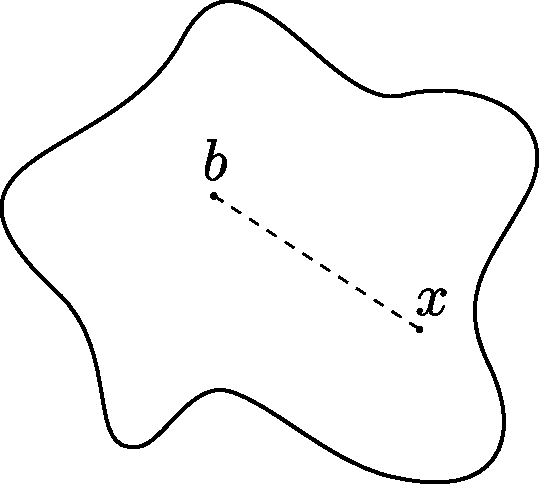
\includegraphics[width=2in]{905/Figures/05-star-shaped.pdf}
\end{center}

Any nonempty convex region is star shaped.
Any star-shaped region $X$ is contractible: A homotopy 
inverse to $X\to\ast$ is given by sending $\ast\mapsto b$. One composite is
perforce the identity. A homotopy from the other composite to the identity
$1_X$ is given by $(x,t)\mapsto tb+(1-t)x$.

So we should expect that $\epsilon:H_*(X)\to\mathbf{Z}$ is an isomorphism 
if $X$ is star-shaped. In fact, using a piece of language that the reader
can interpret:
\begin{prop}
$S_*(X)\to\mathbf{Z}$ is a chain homotopy equivalence.
\end{prop}

		\begin{proof}
		We have maps $S_\ast(X)\xrightarrow{\epsilon}\mathbf{Z}\xrightarrow{\eta}S_\ast(X)$ where $\eta(1)=c_b^0$. Clearly $\epsilon\eta=1$, and the claim is that $\eta\epsilon\simeq1:S_\ast(X)\to S_\ast(X)$. The chain map 
$\eta\epsilon$ concentrates everything at the point $b$: 
$\eta\epsilon\sigma=c_b^n$ for all $\sigma\in\Sin_n(X)$. 
Our chain homotopy $h:S_q(X)\to S_{q+1}(X)$ will actually send simplices to simplices. For $\sigma\in\Sin_q(X)$, define the chain homotopy evaluated on $\sigma$ by means of the following ``cone construction'': $h(\sigma)=b*\sigma$, where
\[
(b*\sigma)(t_0,\ldots,t_{q+1})=t_0b+(1-t_0)\sigma\left(\frac{(t_1,\ldots,t_{q+1})}{1-t_0}\right)\,.
\]
Explanation: The denominator $1-t_0$ makes the entries sum to 1, as they must if we are to apply $\sigma$ to this vector. When $t_0=1$, this isn't defined, but it doesn't matter since we are multiplying by $1-t_0$. So
$(b*\sigma)(1,0,\ldots,0)=b$; this is the vertex of the cone. 

\begin{center}
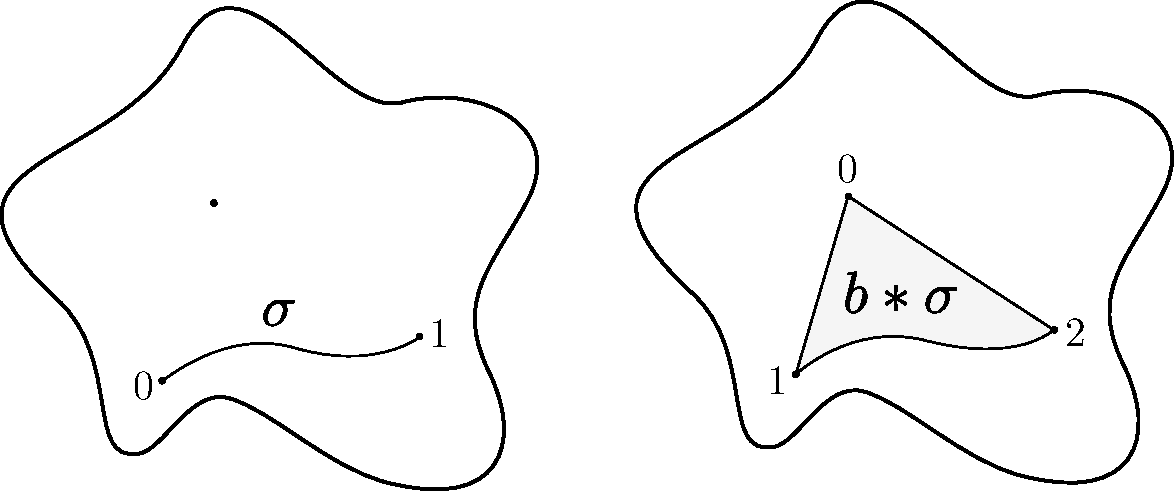
\includegraphics[width=5in]{905/Figures/05-homotopy.pdf}
\end{center}

Setting $t_0=0$, we find
\[
d_0b*\sigma=\sigma\,.
\]
Setting $t_i=0$ for $i>0$, we find
\[
d_ib*\sigma=hd_{i-1}\sigma\,.
\]
Using the formula for the boundary operator, we find
\[
db*\sigma=\sigma-b*d\sigma
\]
\ldots {\em unless} $q=0$, when 
\[
db*\sigma=\sigma-c_b^0\,.
\]
This can be assembled into the equation
\[
db*+b*d=1-\eta\epsilon
\]
which is what we wanted. 		
\end{proof}




% Continue indenting like this.
